\documentclass[11pt,a4paper]{article}
\usepackage[top=3cm, bottom=2cm, left=2cm, right=2cm]{geometry}
\usepackage[utf8]{inputenc}
\usepackage{amsmath, amsfonts, amssymb}
\usepackage{siunitx}
\usepackage[brazil]{babel}
\usepackage{graphicx}
\usepackage[margin=10pt,font={small, it},labelfont=bf, textfont=it]{caption}
\usepackage[dvipsnames, svgnames]{xcolor}
\DeclareCaptionFont{MediumOrchid}{\color[svgnames]{MediumOrchid}}
\usepackage[pdftex]{hyperref}
\usepackage{natbib}
\bibliographystyle{plainnat}
\bibpunct{\textcolor{MediumOrchid}{\textbf{[}}}{\textcolor{MediumOrchid}{\textbf{]}}}{,}{s}{}{}
\usepackage{color}
\usepackage{footnote}
\usepackage{setspace}
\usepackage{booktabs}
\usepackage{multirow}
\usepackage{subfigure}
\usepackage{fancyhdr}
\usepackage{leading}
\usepackage{indentfirst}
\usepackage{wrapfig}
\usepackage{mdframed}
\usepackage{etoolbox}
\usepackage[version=4]{mhchem}
\usepackage{enumitem}
\usepackage{caption}
\usepackage{titlesec}
\usepackage{tcolorbox}
\usepackage{tikz}
\usepackage{LobsterTwo}
\usepackage[T1]{fontenc}
\usepackage{fontspec}
\usepackage{txfonts}
\usepackage[bottom]{footmisc}
\tcbuselibrary{skins,breakable}
\sisetup{output-decimal-marker={.}}

\makeatletter
\def\footnoterule{\kern-3pt\color{MediumOrchid}\hrule\@width0.6\textwidth height 0.8pt\kern2.6pt}
\makeatother

\renewcommand{\footnotelayout}{\itshape\color{MediumOrchid}}

\AtBeginEnvironment{equation}{\fontsize{13}{16}\selectfont}


\titleformat{\section}{\LobsterTwo\huge\color{CarnationPink}}{\thesection.}{1em}{}
\titleformat{\subsection}{\LobsterTwo\huge\color{CarnationPink}}{\thesubsection}{1em}{}
\titleformat{\subsubsection}{\bf\LobsterTwo\Large\color{MediumOrchid}}{\thesubsubsection}{1em}{}


\DeclareCaptionLabelFormat{figuras}{\textcolor{DarkTurquoise}{Figura \arabic{figure}}}
\captionsetup[figure]{labelformat=figuras}

\makeatletter
\renewcommand\tagform@[1]{\maketag@@@{\color{CarnationPink}(#1)}}
\makeatother

\renewcommand{\theequation}{Eq. \arabic{equation}}
\renewcommand{\thefigure}{Fig. \arabic{figure}}
\renewcommand{\thesection}{\textcolor{CarnationPink}{\arabic{section}}}

\setlist[itemize]{label=\textcolor{CarnationPink}{$\blacksquare$}}

\setlist[enumerate]{label=\textcolor{CarnationPink}{\arabic*.}, align=left, leftmargin=1.5cm}


\newcounter{exemplo}

\NewDocumentEnvironment{exemplo}{ O{} }{%
\allowbreak
\setlength{\parindent}{0pt}
  \begin{mdframed}[
  leftline=true,
  topline=false,
  rightline=false,
  bottomline=false,
  linewidth=2pt,
  linecolor=CarnationPink,
  frametitlerule=false,
  frametitlefont=\LobsterTwo\large\color{CarnationPink},
  frametitle={\color{CarnationPink}\LobsterTwo\large #1},
  ]
}{%
  \end{mdframed}
}

\setlength{\fboxsep}{5pt}
\setlength{\fboxrule}{1.5pt}
\usepackage{float}
\renewcommand{\thefootnote}{\alph{footnote}}
\usepackage{url}
\hypersetup{
	colorlinks=true,
	linkcolor=DarkTurquoise,
	filecolor=DarkTurquoise,      
	urlcolor=DarkTurquoise,
	citecolor=DarkTurquoise,
	pdftitle={Especialista em Física da Radioterapia}
}
\pagestyle{fancy}
\fancyhf{}
\renewcommand{\headrulewidth}{0pt}
\rfoot{\color{DarkTurquoise}\thepage \\ \LobsterTwo{\small\textcolor{CarnationPink}{@defDalila}}}

\title{\LobsterTwo\Huge{Radioterapia}}
\author{\LobsterTwo\Large{Radioterapia Intraoperatória}\nocite{*}}
\date{\LobsterTwo\textit{Dalila Mendonça}}
\begin{document}
	\maketitle

\section{Introdução}

	A radioterapia intraoperatória (IORT) é uma abordagem terapêutica em que uma dose alta de radiação é entregue diretamente no local do tumor durante a cirurgia. Isso difere da radioterapia externa convencional, em que a radiação é administrada em sessões diárias ao longo de várias semanas. A IORT é particularmente útil em casos em que é difícil alcançar uma ressecção cirúrgica completa devido à localização do tumor próximo a estruturas críticas que não podem ser completamente removidas.

	Ao irradiar o local do tumor durante a cirurgia, a IORT pode ajudar a controlar a doença de forma mais eficaz. Além disso, a IORT pode ser uma opção viável quando a radioterapia externa já foi administrada e as estruturas críticas atingiram doses máximas toleráveis. A capacidade de visualizar diretamente o leito tumoral durante a cirurgia permite uma precisão maior no direcionamento da radiação para o local desejado, minimizando assim a exposição de tecidos saudáveis adjacentes.A IORT também oferece a vantagem de permitir a proteção direta ou o deslocamento de estruturas sensíveis, como nervos ou vasos sanguíneos, fora do campo de tratamento, reduzindo assim o risco de complicações e efeitos colaterais indesejados.

	É importante ressaltar que, embora haja apoio para o uso da IORT em estudos realizados em instituições específicas e em análises retrospectivas agrupadas, ainda há a necessidade de grandes ensaios clínicos randomizados para fornecer evidências mais robustas sobre sua eficácia em diferentes cenários clínicos.

	A radioterapia intraoperatória (IORT) tem desempenhado um papel importante no tratamento do câncer de mama. Uma das aplicações é a radioterapia parcial acelerada da mama (APBI), que envolve a entrega de uma dose alta de radiação diretamente na cavidade da mastectomia após a cirurgia conservadora da mama. A ideia por trás desse tratamento é proporcionar controle local ao focar a irradiação na área onde o tumor foi removido, uma vez que a recorrência local geralmente ocorre nessa região.

	Um estudo significativo nesse contexto é o ensaio clínico randomizado TARGIT-A, que comparou a IORT como tratamento único à radioterapia convencional de toda a mama após a cirurgia conservadora da mama. Os resultados de acompanhamento de 5 anos mostraram que as taxas de recorrência local no grupo da IORT não foram estatisticamente diferentes do grupo de radioterapia convencional. Além disso, observou-se uma diminuição no número de óbitos não relacionados ao câncer no grupo da IORT, especialmente devido a doenças cardiovasculares. Esses resultados apoiam o uso da IORT como uma opção eficaz em pacientes selecionados com câncer de mama.

	Outra aplicação da IORT no câncer de mama é a substituição da fase de boost durante o curso do tratamento. Tradicionalmente, um boost adicional de radioterapia é administrado após a radioterapia externa da mama para aumentar a dose no leito tumoral. No entanto, a IORT tem sido investigada como uma alternativa para fornecer uma dose de reforço diretamente no local da cirurgia, eliminando assim a necessidade de uma fase adicional de tratamento.

	Uma teoria que pode explicar os resultados positivos da IORT no câncer de mama é a esterilização do fluido da ferida durante a cirurgia com radiação. Acredita-se que a irradiação durante a cirurgia ajude a prevenir o crescimento de células tumorais residuais, reduzindo assim o risco de recorrência local. No entanto, é importante ressaltar que cada caso é único, e a decisão de usar a IORT como parte do tratamento do câncer de mama deve ser feita em conjunto pela equipe médica e o paciente, levando em consideração diversos fatores, como características do tumor, estado clínico e preferências individuais.

	Em alguns casos, a IORT é utilizada em combinação com a EBRT como parte do tratamento abrangente do câncer. Nesse contexto, a EBRT é administrada antes da cirurgia para tratar o tumor primário e reduzir o tamanho do tumor. A IORT é então aplicada durante a cirurgia para fornecer uma dose alta de radiação diretamente no leito tumoral, visando controlar qualquer doença residual ou margens positivas. Nesse cenário, as doses típicas de IORT são:

	\begin{itemize}
		\item 7.5 a 10 Gy para margens negativas ou próximas
		\item 10 a 12,5 Gy para margens positivas
		\item 15 a 20 Gy para doença residual extensa ou tumor não ressecável.
	\end{itemize}

	O status da margem pode ser determinado intraoperatoriamente por meio da patologia tecidual congelada. Em pacientes com doença recorrente que já receberam radioterapia prévia, pode não ser seguro administrar altas doses de EBRT. Nesses casos, doses mais elevadas de IORT (15 a 20 Gy) podem ser administradas para compensar. É importante ressaltar que o planejamento da dose de IORT leva em consideração as estruturas críticas adjacentes, como nervos, vasos sanguíneos e anastomoses cirúrgicas\footnote{As anastomoses cirúrgicas são conexões criadas entre duas estruturas do corpo durante um procedimento cirúrgico. Essas conexões são feitas quando uma parte do corpo precisa ser reconectada a outra, seja para restaurar o fluxo sanguíneo, o fluxo de líquidos ou a continuidade de um órgão.}. O objetivo é garantir que essas estruturas sejam protegidas dentro de limites de dose seguros, minimizando assim os efeitos colaterais adversos. Em alguns casos, as complicações pós-tratamento podem limitar a adequação do paciente para receber IORT, mesmo que inicialmente tenham sido considerados candidatos. Por isso, é essencial uma avaliação cuidadosa e individualizada de cada paciente antes de decidir pela inclusão da IORT em seu plano de tratamento.

\section{Tecnologias e Técnicas para IORT}

	Uma variedade de tecnologias está disponível para fornecer IORT, conforme resumido na \ref{fig:iortTecnologias}. Cada um tem vantagens e desvantagens clínicas e práticas.

	\begin{figure}[h]
		\centering
		\fcolorbox{DarkTurquoise}{white}{%
			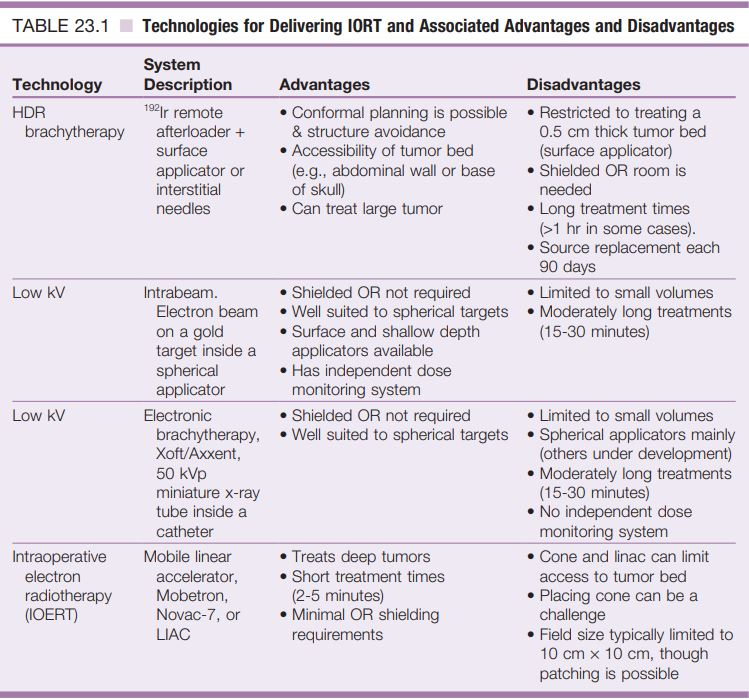
\includegraphics[width=0.8\textwidth]{Imagens/iortTecnologias.JPG}
		}%
		\caption{Tecnologias para fornecimento de IORT e vantagens e desvantagens associadas.}
		\label{fig:iortTecnologias}
	\end{figure}

\subsubsection*{Radioterapia Eletrônica Intraoperatória (IOERT) em Aceleradores Lineares}

	A IOERT é uma técnica de radioterapia que envolve a entrega de uma dose alta de radiação diretamente no leito tumoral durante a cirurgia. Ela utiliza feixes de elétrons, que são partículas carregadas eletricamente, para irradiar o tecido alvo. Os feixes de elétrons são produzidos por um acelerador linear, um equipamento que gera radiação de alta energia para uso terapêutico. No passado, alguns centros possuíam salas de tratamento com linacs dedicadas à IOERT, que também poderiam ser usadas como salas de cirurgia. No entanto, com o avanço da tecnologia, foram desenvolvidos linacs móveis que podem ser transportados para diferentes salas de cirurgia, permitindo uma maior acessibilidade e flexibilidade no uso da IOERT.

	A AAPM é uma organização profissional que busca promover a qualidade e a segurança da prática da física médica em radioterapia. Ela estabelece grupos de trabalho (TG) compostos por especialistas na área para desenvolver diretrizes e recomendações sobre diversos tópicos relacionados à radioterapia, incluindo a IOERT. O AAPM TG-48 foi publicado em 1995 e tratava especificamente da IOERT. Posteriormente, em 2006, o AAPM TG-72 foi publicado para abordar a IOERT com linacs móveis, substituindo em grande parte as diretrizes anteriores.

	Existem três unidades móveis de IOERT disponíveis comercialmente: Mobetron (Intraoperative Medical Systems, Inc., Santa Clara, CA), Novac-7 (Hitesys SRL, Aprilia, Itália) e LIAC (Itália). O Mobetron (\ref{fig:iortIntrabeam}) foi utilizado pela primeira vez na Universidade da Califórnia em São Francisco em 1997 e é o sistema mais amplamente utilizado nos Estados Unidos. Ele é descrito em detalhes no AAPM TG-72, embora o sistema tenha sido modificado desde a publicação desse relatório. 


	\begin{figure}[h]
		\centering
		\fcolorbox{DarkTurquoise}{white}{%
			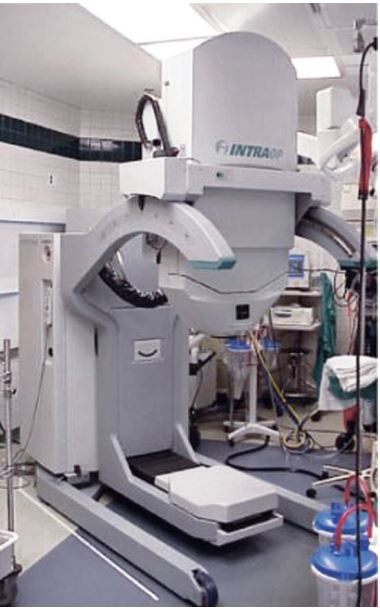
\includegraphics[width=0.6\textwidth]{Imagens/iortMobile.JPG}
		}%
		\caption{IOERT -- linac Móvel Mobetron (IntraOp Inc.) gerando elétrons de 6 a 12 MeV. O linac se acopla a um cone aplicador de metal no paciente usando um mecanismo “soft-docking”. O beam stop (inferior) protege contra contaminação de fótons, tornando possível a implantação em salas de cirurgia não blindadas.}
		\label{fig:iortMobile}
	\end{figure}

	O Mobetron utiliza um linac compacto operando na frequência de 10 GHz da banda X (a maioria dos outros linacs são aceleradores da banda S a 3 GHz, tornando-os aproximadamente três vezes maiores). Atualmente, ele fornece feixes de elétrons nas energias de 6 MeV, 9 MeV e 12 MeV em altas taxas de dose (aproximadamente 10 Gy/min), o que facilita os procedimentos na sala de cirurgia (OR). A distância fonte-superfície efetiva (SSD) é de 50 cm. O linac é montado em um braço em forma de C que permite posicioná-lo com uma inclinação de $\pm$\ang{45} (no eixo esquerda-direita para um paciente com a cabeça voltada para o gantry) e uma inclinação da cabeça de $+$10 a -\ang{30} (eixo superior-inferior). Isso possibilita um posicionamento mais fácil durante o procedimento, embora o posicionamento ainda possa ser um desafio. 

	Aplicadores metálicos são usados para colimar o feixe de elétrons. Os tamanhos dos aplicadores variam de círculos de 3 cm a 10 cm, disponíveis em incrementos de 0.5 cm. A extremidade ddo aplicador pode ser plana ou inclinada em em \ang{15} ou \ang{30}. A inclinação proporciona melhor acesso a algumas regiões, como a parede pélvica. Tipicamente, utiliza-se uma margem de 1 cm ao redor da área tumoral envolvida. Durante o procedimento, o aplicador adequado (estéril) é selecionado e fixado na mesa da sala de cirurgia com um \footnote{O grampo Buckwalter é um dispositivo cirúrgico usado para realizar anastomoses ou conexões entre tecidos durante procedimentos cirúrgicos.}.

	Após o posicionamento do aplicador no paciente, o linac é alinhado à face superior do aplicador. O Mobetron utiliza um mecanismo de "acoplamento suave" baseado em laser para esse propósito, enquanto os sistemas Novac-7 e LIAC utilizam acoplamento rígido para fixar o aplicador no linac.  O acoplamento suave significa que o acelerador está fisicamente desacoplado do aplicador no paciente, reduzindo assim a chance de interação direta com o paciente. 
	
	O IOERT é uma abordagem útil em situações em que a ressecção cirúrgica completa do tumor é difícil devido à sua localização próxima a estruturas críticas ou em casos de recorrência tumoral após tratamento prévio com radioterapia externa. Ele oferece a vantagem de irradiar diretamente o leito tumoral durante a cirurgia, permitindo uma visualização direta e a possibilidade de proteger ou mover estruturas sensíveis fora do campo de tratamento. Estudos clínicos e ensaios randomizados, como o TARGIT-A trial, têm demonstrado resultados encorajadores para o uso do IOERT em pacientes com câncer de mama, especialmente na radioterapia parcial acelerada da mama (APBI).

	Em IOERT, é crucial proteger as estruturas críticas adjacentes ao tumor que está sendo irradiado. O uso de blindagens de chumbo cobertos por gaze embebida em soro fisiológico é uma prática comum para reduzir a dose nessas estruturas. O chumbo tem propriedades de atenuação que podem reduzir significativamente a dose de radiação transmitida em 90\% para além do tumor. É importante considerar a espessura adequada do escudo de chumbo para garantir uma redução eficaz na dose. A regra do "Rp/10" é frequentemente usada como um guia para determinar a espessura mínima necessária da blindagem. Essa regra indica que a espessura da blindagem de chumbo deve ser pelo menos 10 vezes maior que o alcance prático (Rp) do feixe de elétrons. Isso ajuda a garantir que a maioria dos elétrons seja atenuados pela blindagem antes de atingir as estruturas críticas.

	Na IOERT, as prescrições geralmente são definidas na linha isodose de 90\%. Além disso, o uso de materiais de "bolus" (com 0.5 cm ou 1.0 cm de espessura) pode ser necessário em certos casos para ajustar a distribuição de dose. O bolus é colocado na superfície do paciente durante o tratamento para aumentar a dose na região superficial ou reduzir a profundidade de penetração do feixe de elétrons. Isso pode ser útil para garantir que a dose seja entregue com maior precisão ao tumor e minimizar a dose em tecidos saudáveis adjacentes.

	A contagem adequada dos dispositivos de proteção e bolus utilizados durante o procedimento é importante para garantir a rastreabilidade e segurança do tratamento. Isso inclui registrar o uso desses dispositivos nos registros de instrumentação da sala cirúrgica, garantindo que nenhum item seja esquecido no paciente após o procedimento.

	A fase de aceitação e comissionamento do equipamento de IOERT é um processo crítico e minucioso que visa garantir a confiabilidade e a precisão dos resultados obtidos. As diretrizes fornecidas pela AAPM TG-72 são fundamentais para orientar esse processo. Durante essa fase, são realizadas várias tarefas de medição que abrangem diferentes aspectos do equipamento e do tratamento. Uma das principais tarefas é a avaliação da dose em profundidade (PDD), que fornece informações essenciais sobre como a radiação se distribui ao longo do tecido. Através dessa medição, é possível determinar a quantidade de dose absorvida em diferentes profundidades, o que é fundamental para ajustar a dose entregue ao paciente de forma precisa e adequada. 

	Além disso, são realizadas medições de perfil de dose, que fornecem informações detalhadas sobre a distribuição espacial da radiação. Os fatores do aplicador também são determinados durante o processo de comissionamento. Esses fatores são relativos a um aplicador padrão de 10 cm,  normalmente especificados em dmax e frequentemente medidos com um diodo de elétrons, e são utilizados para fazer os ajustes necessários na dosagem. Eles levam em consideração as características do aplicador em relação à dose absorvida pelo tecido, garantindo uma entrega precisa da radiação. Outro aspecto importante é a medição dos fatores de espaço aéreo. Como nem sempre é possível posicionar os aplicadores em contato direto com o tecido, é necessário levar em consideração os efeitos do espaço aéreo entre o aplicador e o tecido. Esses fatores garantem uma correção adequada na dosagem, levando em conta as condições específicas de cada caso.

	Além das medições mencionadas, também é essencial realizar a medição dos vazamentos fora do aplicador. Essa medição visa verificar se há radiação indesejada sendo emitida fora da área de tratamento, o que pode comprometer a segurança do paciente. É importante avaliar e quantificar esses vazamentos para garantir que estejam dentro de limites aceitáveis. Por exemplo, os vazamentos fora do aplicador podem atingir até 25\% da dose prescrita. Finalmente, a calibração da saída do equipamento de IOERT é realizada de acordo com as diretrizes estabelecidas pela AAPM TG-51 ou protocolos equivalentes. A calibração adequada da saída é essencial para garantir que as doses prescritas sejam entregues com precisão e confiabilidade.

	No caso específico do equipamento Novac-7, é importante estar ciente dos efeitos de recombinção iônica. Devido à alta dose por pulso ($>$10 mGy/pulso), esses efeitos podem se tornar significativos e resultar em erros na dose entregue de até 20\%. Portanto, a recomendação é evitar o uso de protocolos de calibração de câmaras de ionização nesse regime. Alternativamente, os dosímetros de Fricke podem ser utilizados como uma opção confiável para medir a dose absorvida nessas condições desafiadoras. Os dosímetros de Fricke são dispositivos químicos capazes de fornecer informações precisas sobre a dose de radiação absorvida pelo meio, mesmo em situações com altas doses por pulso.

	Os linacs móveis são equipamentos que utilizam elétrons de baixa energia (12 MeV) para realizar o tratamento radioterápico durante uma cirurgia. Devido à baixa energia, os requisitos de blindagem são mínimos em comparação com os linacs convencionais. No entanto, ainda é necessário considerar o vazamento e o espalhamento de fótons produzidos pelos linacs móveis ao posicionar o equipamento em uma sala de cirurgia, que normalmente não possui blindagem adequada. O Mobetron, um dos linacs móveis mais utilizados, possui um stop beam atrás do paciente para interceptar fótons indesejados, mas ainda existem componentes extrafocais que devem ser considerados.

	Um estudo de blindagem realizado por Krechtov et al.10 para a unidade Mobetron concluiu que cargas de trabalho de 5 a 6 pacientes por semana podem ser acomodadas nos limites de uma sala de cirurgia típica, mas é importante realizar cálculos e levantamentos de blindagem específicos para cada instalação. Além disso, ao considerar a carga de trabalho, é necessário levar em conta o tempo de aquecimento diário e o controle de qualidade, que podem ter uma duração igual ou maior do que o tempo real de irradiação utilizado nos tratamentos.

	É importante destacar que investigações mostraram que abaixo de 12 MeV há pouca contaminação por nêutrons, o que permite que esse componente seja ignorado nas considerações de blindagem. Caso a blindagem não seja suficiente, é possível utilizar mais de uma sala de cirurgia ou implementar barreiras móveis para garantir a segurança dos profissionais e pacientes. Devido ao grande número de unidades monitoras utilizadas durante o tratamento, muitas vezes é necessário colocar o linac móvel em uma sala de blindagem durante a fase de comissionamento.

	Além dos requisitos de blindagem, outras considerações devem ser levadas em conta ao utilizar um linac IOERT em uma sala de cirurgia, como a disponibilidade de energia adequada para o funcionamento do equipamento e a capacidade de carga estrutural dos pisos para suportar o peso do linac e de outros equipamentos adicionais.


\subsubsection*{Baixo KV e Braquiterapia Eletrônica}

	Existem atualmente dois dispositivos de raios-X de baixa energia (kV) disponíveis no mercado para o tratamento de radioterapia intraoperatória (IORT). O comitê de tecnologia emergente da ASTRO publicou um relatório em 2010 que analisa essas tecnologias. Relatórios completos de grupos de trabalho sobre esses sistemas estão ausentes, mas informações sobre calibração e garantia da qualidade podem ser encontradas no Relatório 152 da AAPM e na resposta de 2007 da AAPM ao pedido da Conference of Radiation Control Program Directors, Inc. (CRCPD) para recomendações sobre as regulamentações do modelo do CRCPD para braquiterapia eletrônica. O TG-182 da AAPM sobre garantia da qualidade da braquiterapia eletrônica foi desenvolvido. Embora os sistemas compartilhem algumas semelhanças na forma como os raios-X são produzidos (uma fonte de elétrons de baixa energia acelerada para um alvo de metal), eles diferem significativamente em suas dimensões físicas e métodos de aplicação.
	
	
	Um desses dispositivos é o Intrabeam, desenvolvido pela Carl Zeiss Surgical em Oberkochen, Alemanha. Embora tenha sido originalmente desenvolvido para o tratamento cerebral, atualmente é amplamente utilizado no tratamento de câncer de mama. O Intrabeam é especialmente adequado para irradiar cavidades quase esféricas, como aquelas resultantes de cirurgias conservadoras de mama.

	O Intrabeam (\ref{fig:iortIntrabeam}) opera acelerando um feixe de elétrons até a extremidade de um tubo de 10 cm, onde colide com um alvo de ouro de 3,2 mm de diâmetro, produzindo raios-X que se distribuem aproximadamente de forma esférica. Na extremidade do dispositivo, é acoplado um aplicador esférico de plástico de polieterimida, disponível em diferentes tamanhos, que varia de 1.5 cm a 5 cm em incrementos de 0,5 cm. Geralmente, os aplicadores de 3 cm a 5 cm são utilizados com mais frequência. A unidade do Intrabeam é montada em um suporte de chão que permite um posicionamento preciso em seis graus de liberdade. Durante o procedimento, a cavidade cirúrgica é fechada ao redor do aplicador com o uso de sutura, e a pele é retraída para proteção adequada. É importante garantir que o tecido se ajuste perfeitamente ao aplicador, o que pode ser verificado com a ajuda de ultrassom. A dose de radiação na pele pode ser medida utilizando filmes radiocrômicos ou dosímetros OSLD colocados em embalagens estéreis.

	\begin{figure}[h]
		\centering
		\fcolorbox{DarkTurquoise}{white}{%
			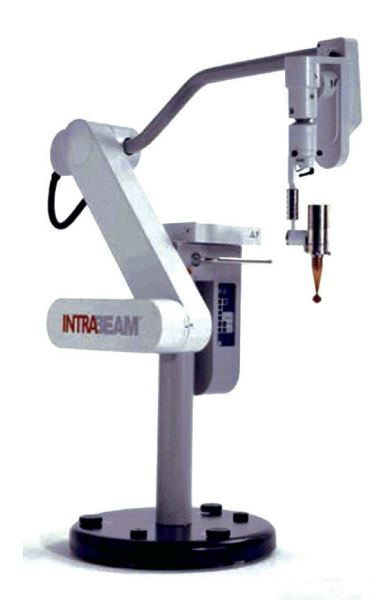
\includegraphics[width=0.7\textwidth]{Imagens/iortIntrabeam.JPG}
		}%
		\caption{O dispositivo Intrabeam (Carl Zeiss Surgical, Oberkochen, Alemanha). Um feixe de elétrons de 50 kV é acelerado em um alvo de ouro no aplicador para produzir uma distribuição de dose de raios X que é aproximadamente esfericamente uniforme.}
		\label{fig:iortIntrabeam}
	\end{figure}

	Em relação à dose prescrita, geralmente é recomendado um valor de 5 Gy a uma profundidade de 1 cm, o que resulta em uma dose de aproximadamente 20 Gy na superfície da pele, dependendo do tamanho do aplicador utilizado. O tempo de tratamento varia de 15 a 30 minutos. Normalmente, não é necessária uma blindagem interna adicional, a menos que o aplicador esteja localizado a menos de 1 cm de uma costela ou parede torácica, o que pode ocorrer em pacientes com baixa espessura de tecido ou lesões mais centrais. Devido ao uso de baixa energia nos raios-X, o Intrabeam não requer uma sala de operações blindada.

	Além do Intrabeam, outro dispositivo de braquiterapia eletrônica utilizado na IORT, especialmente no tratamento de câncer de mama, é o Xoft Axxent, desenvolvido pela Xoft Inc. em Fremont, Califórnia. Esse sistema utiliza um tubo de raios-X em miniatura (2,2 mm de diâmetro por 10 mm de comprimento) inserido em um cateter refrigerado a água. Essa fonte de braquiterapia eletrônica tem uma vida útil de aproximadamente 2,5 horas e é projetada para ser descartável após o uso. O tubo de raios-X opera em até 50 kV e possui um alto nível de filtragem, proporcionando uma distribuição radial de dose semelhante a uma fonte de baixa energia para braquiterapia. Para o tratamento de mama, o sistema Xoft é usado em conjunto com um aplicador de balão de diferentes tamanhos (de 3 cm a 6 cm) para tratar tecidos a uma profundidade de 1 a 2 cm. Esse aplicador de balão pode ser utilizado tanto para um tratamento IORT de dose única, como para a administração de tratamentos fracionados se o balão for deixado na cavidade após a cirurgia. Em relação aos tratamentos fracionados, geralmente são administradas cerca de 10 frações de 3,4 Gy cada, duas vezes ao dia.

	É importante mencionar que ambos os sistemas de braquiterapia eletrônica, Intrabeam e Xoft, têm suas próprias características e aplicadores específicos, que podem estender seu uso além do tratamento de câncer de mama. O Intrabeam possui aplicadores de superfície adicionais para tratamentos pélvicos/abdominais e tratamentos cutâneos, enquanto o sistema Xoft possui outros aplicadores, como aplicadores de retalho (como o aplicador HAM) para tratamentos em outras regiões do corpo, cones de superfície e aplicadores planares expansíveis para cirurgias laparoscópicas.

\subsubsection*{Braquiterapia de Alta Taxa de Dose}

	A IORT é uma técnica avançada de radioterapia que permite a administração de altas doses de radiação diretamente no local do tumor durante a cirurgia. Uma das abordagens para realizar a IORT é utilizando a braquiterapia de alta taxa de dose (HDR), na qual aplicadores de superfície são colocados no paciente e possuem tubos guia pelos quais a fonte de radiação HDR é deslocada.

	Existem diferentes tipos de aplicadores utilizados na IORT baseada em HDR. Um exemplo é o aplicador HAM (Harrison-Anderson-Mick), que consiste em uma folha de silicone com 8 mm de espessura contendo tubos guia espaçados a cada 10 mm. Outro exemplo é o aplicador Freiburg Flap, que emprega uma estrutura de esferas interconectadas em formato de malha. Esses aplicadores podem ser ajustados no tamanho necessário durante o procedimento cirúrgico.

	Uma das vantagens da IORT baseada em HDR é sua capacidade de tratar áreas tumorais extensas e alcançar regiões de difícil acesso, como a parede pélvica lateral. Durante o procedimento, um plano de tratamento é selecionado a partir de um conjunto de planos predefinidos, que são otimizados para garantir uma distribuição uniforme da dose na profundidade desejada. A dose prescrita geralmente é estabelecida a uma profundidade de 0,5 cm no centro do aplicador.

	É importante ressaltar que a IORT baseada em HDR é frequentemente utilizada para tratar tecidos superficiais, embora alguns centros tenham explorado a utilização da braquiterapia intersticial para tratar tumores mais profundos que 0,5 cm. Para proteger estruturas críticas durante o tratamento, discos de chumbo com aproximadamente 3 mm de espessura podem ser colocados.

	Além das considerações técnicas, é essencial levar em conta as necessidades de infraestrutura para a realização da IORT baseada em HDR. Uma sala de cirurgia com blindagem adequada é requerida, devido à alta taxa de dose utilizada e à necessidade de proteger a equipe médica e os pacientes dos efeitos nocivos da radiação. O tempo de tratamento também pode ser mais longo em comparação com outras modalidades de radioterapia, o que requer planejamento adequado em termos de anestesia e monitoramento.

	No que diz respeito aos aspectos de qualidade e segurança, é essencial seguir diretrizes e protocolos estabelecidos. O documento de referência AAPM TG-59 fornece orientações gerais sobre o tratamento de braquiterapia de alta taxa de dose, embora não seja específico para a IORT. É fundamental realizar testes rigorosos de garantia de qualidade dos equipamentos e dos procedimentos. A equipe médica também deve passar por treinamentos regulares em procedimentos de segurança e emergência, incluindo ações a serem tomadas em caso de falha do dispositivo de radiação.

	É importante destacar que a IORT baseada em HDR tem demonstrado eficácia no tratamento de tumores, oferecendo a vantagem de administrar doses elevadas de radiação diretamente no local afetado durante a cirurgia. A técnica continua a evoluir com o avanço tecnológico e com pesquisas adicionais, resultando em aprimoramentos contínuos para melhorar os resultados e a segurança dos pacientes submetidos a esse tipo de tratamento.

	É essencial que pacientes e profissionais de saúde trabalhem em conjunto para entender os benefícios, riscos e possibilidades terapêuticas da IORT baseada em HDR, garantindo uma abordagem personalizada e eficaz para cada caso clínico específico.

\section{Considerações sobre Segurança, Equipe e Sala de Cirurgia}

	A radioterapia intraoperatória (IORT) é um procedimento que requer considerações especiais devido ao ambiente em que é realizado, a sala de operações (OR). Uma das principais preocupações é a necessidade de um ambiente estéril, uma vez que a contaminação pós-operatória é uma das principais causas de complicações em cirurgias. Portanto, é crucial garantir que todo o equipamento utilizado na IORT seja estéril.

	Os aplicadores de IOERT, por exemplo, podem ser esterilizados de diferentes maneiras, dependendo do material de construção. Aplicadores metálicos podem ser esterilizados por calor ou luz UV, enquanto aplicadores feitos de alumínio ou polimetilmetacrilato (PMMA) podem ser esterilizados com etanol gasoso. É importante ressaltar que o uso repetido de esterilização por etanol gasoso em aplicadores de PMMA pode levar a rachaduras no material. Já os aplicadores de HDR também devem ser estéreis e podem exigir um procedimento de esterilização caso sejam abertos para inspeção e testes antes do procedimento.

	Além da necessidade de um ambiente estéril, é fundamental que toda a equipe envolvida na IORT esteja bem treinada nos protocolos de campos estéreis e na manutenção da esterilidade na sala de operações. Nesse sentido, a Associação de Enfermeiros Perioperatórios Registrados (AORN) desenvolveu diretrizes que enfatizam a importância da comunicação e do trabalho em equipe, incluindo a equipe de radioterapia oncológica. A colaboração estreita entre os oncologistas radioterapeutas e os cirurgiões é essencial para identificar com precisão a área a ser tratada e avaliar quaisquer estruturas em risco.

	Além disso, é crucial que a equipe de entrega, composta por médicos, enfermeiros e técnicos, trabalhe em conjunto para posicionar corretamente os aplicadores e, no caso da IOERT, realizar o acoplamento dos pacientes. Em alguns casos, pode ser necessário reposicionar o paciente para garantir a precisão do tratamento. É importante ressaltar que a segurança do paciente é uma prioridade e, portanto, toda a equipe deve receber treinamento adequado em relação aos princípios da administração de radiação e aos aspectos de segurança.

	A cooperação e a comunicação eficazes entre todas as partes envolvidas são fundamentais para garantir a precisão e a qualidade dos tratamentos de IORT, bem como a segurança dos pacientes. Além disso, é importante destacar que a constante atualização e revisão das diretrizes e protocolos é essencial para assegurar que as práticas de IORT estejam alinhadas com as melhores evidências científicas disponíveis.

\bibliography{ref.bib}
\end{document}